%!TEX root=../main.tex

%$Id: sec8-con.tex 87 2011-11-01 20:53:53Z weiwei $

\vspace{-3.5em}

\begin{IEEEbiography}[{\vspace{-2em}\includegraphics[width=0.8in,height=1in,clip,keepaspectratio]{photos/jie.jpg}}]{Jie Zhu} is currently studying for Master degree of Computer Science in Graduate School at Shenzhen, Tsinghua University. She received her Bachelor degree in Beijing University of Posts and Telecommunications. Her current research interests include verifiable data search and privacy.
\end{IEEEbiography}

\vspace{-5.5em}

\begin{IEEEbiography}[{\vspace{-1em}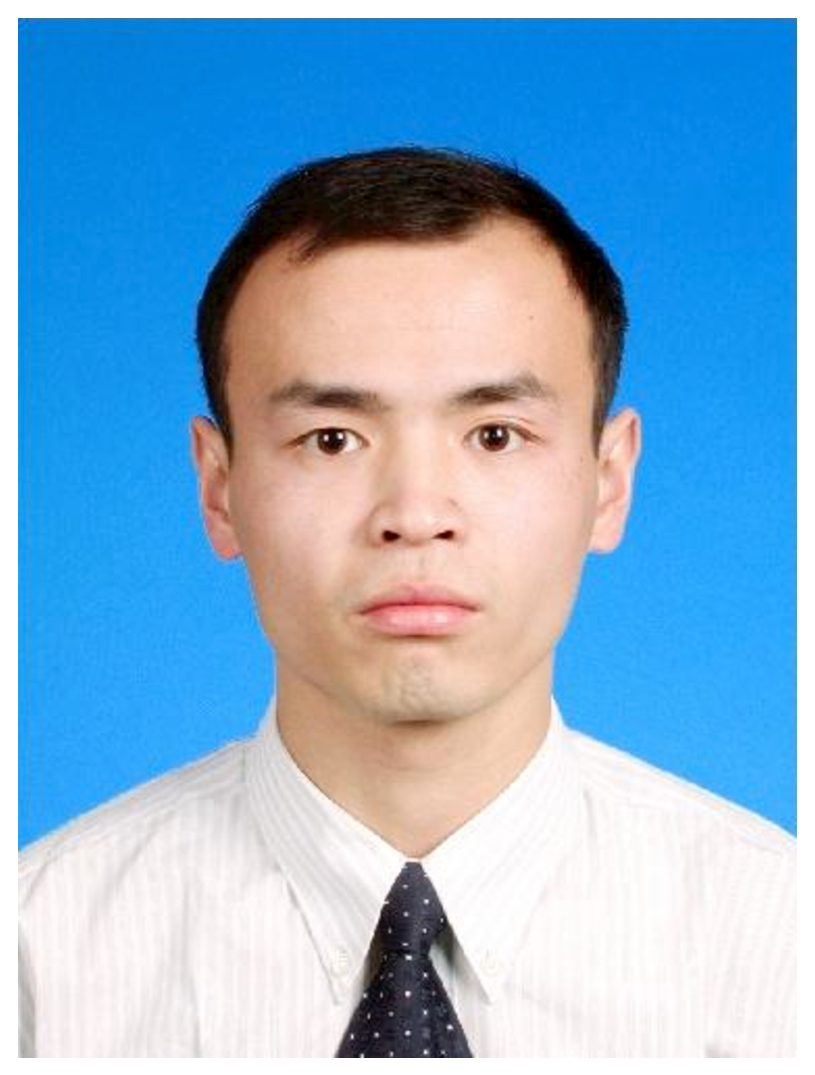
\includegraphics[width=0.8in,height=1in,clip,keepaspectratio]{photos/qi.eps}}]{Qi Li} received his Ph.D. degree from Tsinghua University. Now he is an associate professor of Graduate School at Shenzhen, Tsinghua University. He has ever worked at ETH Zurich, the University of Texas at San Antonio, The Chinese University of Hong Kong, Chinese Academy of Sciences, and Intel.
His research interests are in network and system security, particularly in Internet and cloud security, mobile security, and big data security. He is currently an editorial board member of IEEE TDSC.%, and has served on the organization or program committees of numerous conferences.
\end{IEEEbiography}

\vspace{-3.5em}

\begin{IEEEbiography}[{\vspace{-1em}\includegraphics[width=0.8in,height=1in,clip,keepaspectratio]{photos/cong.jpeg}}]{Cong Wang} received the PhD degree in electrical and computer engineering from the Illinois Institute of Technology, in 2012. He is an assistant professor in the Computer Science Department, City University of Hong Kong. He worked at the Palo Alto Research Center in the summer of 2011. His research interests include the areas of cloud computing security, with current focus on secure data outsourcing and secure computation outsourcing in public cloud.
\end{IEEEbiography}

\vspace{-3.5em}
\begin{IEEEbiography}[{\vspace{-1em}\includegraphics[width=0.8in,height=1in,clip,keepaspectratio]{photos/yuan.jpg}}]{Xingliang Yuan} received the B.S. degree from Nanjing University of Posts and Telecommunications in 2008, the M.S. degree from Illinois Institute of Technology in 2009, both in Electrical Engineering, and the Ph.D. degree in Computer Science from City University of Hong Kong in 2016. He is a Lecturer with the Faculty of Information Technology at Monash University. His research interests include cloud security, NFV security, and privacy-aware computing.
\end{IEEEbiography}

\vspace{-3.5em}

%\vspace{-30em}
\begin{IEEEbiography}[{\vspace{-1em}\includegraphics[width=0.8in,height=1in,clip,keepaspectratio]{photos/qian.eps}}]{Qian Wang} received the B.S. degree from Wuhan University, Wuhan, China, in 2003, the M.S. degree from Shanghai Institute of Microsystem and Information Technology (SIMIT), Chinese Academy of Sciences, Shanghai, China, in 2006, and the Ph.D. degree from Illinois Institute of Technology, Chicago, IL, USA, in 2012, all in electrical engineering.He is a Professor with the School of Computer Science, Wuhan University. His research interests include wireless network security and privacy, cloud computing security, and applied cryptography. He is currently an editorial board member of IEEE TIFS.
\end{IEEEbiography}

\vspace{-3.5em}

\begin{IEEEbiography}[{\vspace{-1em}\includegraphics[width=0.8in,height=1in,clip,keepaspectratio]{photos/kuiren.eps}}]{Kui Ren} received the Ph.D. degree from the Worcester Polytechnic Institute. He is currently a Professor of Institute of Cyber Security Research in Zhejiang University. His current research interests span cloud and outsourcing security, wireless and wearable system security, and human-centered computing. He currently serves as an Associate Editor of IEEE TDSC, TMC, IEEE TSG, IEEE Wireless Communications, IEEE IoT Journal, Pervasive and Mobile Computing (Elsevier), and The Computer Journal (Oxford).


%He currently serves as an Associate Editor of various premier journals, e.g., IEEE TMC, IEEE TDSC.  %e.g., the IEEE Transactions on Dependable and Secure Computing and the IEEE Transactions on Mobile Computing.
%He was a recipient of the NSF CAREER Award in 2011 and the Sigma Xi/IIT Research Excellence Award in 2012. He has authored 135 peer-reviewed journal and conference papers and received several best paper awards, including the IEEE ICNP 2011.
%He currently serves as an Associate Editor of the IEEE Transactions on Dependable and Secure Computing, the IEEE Transactions on Mobile Computing, the IEEE Wireless Communications, the IEEE Internet of Things Journal, the IEEE Transactions on Smart Grid, Pervasive and Mobile Computing (Elsevier), and The Computer Journal (Oxford).
\end{IEEEbiography}
